Write according to vectors:

$$\vec{a}_R = \vec{a}_I \underbrace{-\vec{\omega}\times\left(\vec{\omega} \times \vec{r}\right)}_{\parbox{1.5cm}{\scriptsize  \centering  centrifugal \\ acceleration}} \underbrace{- 2\vec{\omega} \times \vec{v}_R}_{\parbox{1.5cm}{\scriptsize  \centering  Coriolis \\ acceleration}} $$

This result is general for a movement even outside of plane.

\subsection{Exact treatment}

Given an rotation system $R$ with a constant angular velocity $\vec{\omega} = \omega \hat{z}_I$.

Axis $z_R$ and $z_I$ are same. An angle between $x_I$ and $x_R$ is $\theta = \omega t$.

\begin{center}
	\includegraphics[width=\linewidth]{./lect7/pic1.png}
\end{center}

We can see 

$$\begin{cases*}
x_I =  x_R \cos \omega t - y_R \sin \omega t \\
y_I =  x_R \sin \omega t + y_R \cos \omega t \\
\end{cases*}$$

This is right for any vector and can be used to switch between systems $R$ and $I$.

$$\begin{cases*}
(v_R)_{x_I} =  \dot{x}_R \cos \omega t - \dot{y_R} \sin \omega t \\
(v_R)_{y_I} =  \dot{x}_R \sin \omega t + \dot{y_R} \cos \omega t \\
\end{cases*}$$

\textbf{Note:} This isn't velocity in system $I$, those are components of velocity in system $R$ for axis of system $I$.


$$\begin{cases*}
(a_R)_{x_I} =  \dot{x}_R \cos \omega t - \dot{y_R} \sin \omega t \\
(a_R)_{y_I} =  \ddot{x_R} \sin \omega t + \ddot{y_R} \cos \omega t \\
\end{cases*}$$

To find $v_I$ we derive position vector:

$$\frac{d\vec{r}}{dt} = \hat{x}_I\dot{x}_I + \hat{y}_R\dot{y}_R$$

$$\frac{dx_I}{dt} = \dot{x}_I = \underbrace{\dot{x}_R \cos \omega t - \dot{y}_R \sin \omega t}_{\parbox{1.5cm}{\scriptsize  \centering  $(v_R)_{x_I}$  } } \underbrace{ - \omega x_R \sin \omega t  - \omega y_R \cos \omega t}_{\parbox{1.5cm}{\scriptsize  \centering  $(-\omega y_I)_{x_I}$} }$$

$$\frac{dy_I}{dt} = \dot{y}_I =  \underbrace{\dot{x}_R \sin \omega t  + \dot{y}_R \cos \omega t}_{\parbox{1.5cm}{\scriptsize  \centering  $(v_R)_{y_I}$ } } \underbrace{  + \omega x_R \cos \omega t- \omega y_R \sin \omega t}_{\parbox{1.5cm}{\scriptsize  \centering   $(\omega x_I)_{y_I}$} }  $$

Left term is velocity, right is cross product of $\omega$ and $\vec{r}_I$ ($- \omega y_I \hat{x}_I + \omega x_I \hat{y}_I$, $\omega$ has only $z$ component, and $\vec{r}$ has only $x$ and $y$).

$$\vec{v}_I = \left(\frac{d\vec{r}}{dt}\right)_I =  \left(\frac{d\vec{r}}{dt}\right)_R + (\vec{\omega} \times \vec{r}_I)_R$$

It is right for any vector. If we replace position with velocity, we acquire an equation for acceleration: 
\begin{align*}
\omit\rlap{$\vec{a}_I = \bigg(\frac{d\vec{v}_I}{dt}\bigg)_I =  \bigg(\frac{d\vec{v}_I}{dt}\bigg)_R + (\vec{\omega} \times \vec{v}_I)_R$} \\
=& \bigg\{ \frac{d}{dt}\bigg[ &\bigg( \frac{d\vec{r}}{dt} \bigg)_R \enspace +\enspace& ( \vec{\omega} \times \vec{r} )_R \bigg] \bigg\}_R + \bigg\{ \vec{\omega} \times \bigg[ &\bigg(\frac{d\vec{r}}{dt}\bigg)_R \enspace +\enspace &( \vec{\omega} \times \vec{r})_R & \bigg] \bigg\}_R \stackrel{\omega = const}{=} \\
= &  &\vec{a}_R \enspace +\enspace& \vec{\omega} \times \vec{v}_R + &  \vec{\omega} \times \vec{v}_R \enspace +\enspace& \omega \times ( \vec{\omega} \times \vec{v}_R )& = \\
\omit\rlap{$=  \vec{a}_R - \vec{\omega} \times ( \vec{\omega} \times \vec{r} ) - 2 \vec{\omega} \times \vec{v}_R$}
\end{align*}


\begin{center}
	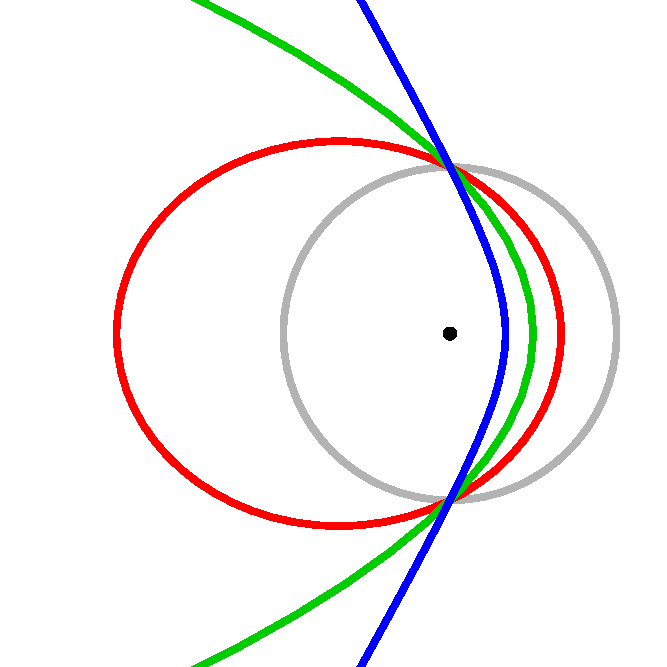
\includegraphics[width=0.7\linewidth]{./lect7/pic2.png}
\end{center}

Free fall on Earth includes a centrifugal acceleration, so a fall is not exactly in direction to center of Earth, but it is negligible.